% import du préambule
\documentclass[12pt,a4paper]{article}
\usepackage[utf8]{inputenc}
\usepackage[french]{babel}
\usepackage[T1]{fontenc}
\usepackage{amsmath}
\usepackage{amsfonts}
\usepackage{amssymb}
\usepackage{array}
\usepackage[table,xcdraw]{xcolor}
\usepackage{amsthm}
\usepackage{graphicx}
\usepackage{caption}
\usepackage[fs]{umons-coverpage}
\usepackage[margin=1.2in]{geometry}
\usepackage[inkscapelatex=false]{svg}
\usepackage{subfiles}
\usepackage{hyperref}
\usepackage{subcaption}
\usepackage{titlesec}
\usepackage{float}
\usepackage{multirow}
\usepackage{listings}
\usepackage{booktabs}
\usepackage{enumitem}
\usepackage{algorithm}
\usepackage{algpseudocode}
\usepackage{transparent}


% définir de nouvelle commande , utiles si on écrit plusieurs fois la même choses
\newcommand{\BN}{ \beta \mathbb{N}}
\newcommand{\N}{\mathbb{N}}
\newcommand{\R}{\mathbb{R}}
\renewcommand{\O}{\mathcal{O}}
\renewcommand{\t}{\text}




% Paramètres de la page de garde.
\title{Prédiction du score de Macron au 2nd tour des élections 2022}
\author{Roland , Stela , Prestonne}
\institute[]{%
  Université de Mons
  \\[2ex]
  
\includegraphics[height=4ex]{beamer_config/images/logoumons.jpg}\hspace{2em}%
  \raisebox{-1ex}{
\includegraphics[height=6ex]{beamer_config/images/logofs.jpg}}
} 
\date{ \today } 
 


\begin{document}

\begin{frame} 
    \titlepage
\end{frame}

\begin{frame}
    \tableofcontents
\end{frame}


\section{Exploration des données}
\input{sections/ExplorationDonnées}

\section{Méthodologie}
\section{Méthodologie}

\subsection*{Prétraitement des données}

Avant l'entraînement des modèles, plusieurs étapes de préparation ont été réalisées :

\begin{itemize}
  \item \textbf{Nettoyage} : suppression des variables non informatives (identifiants, constantes), traitement des valeurs manquantes (par suppression ou imputation simple).
  \item \textbf{Conversion des types} : certaines colonnes contenant des virgules comme séparateur décimal ont été converties en format numérique.
  \item \textbf{Encodage des variables catégorielles} : les variables qualitatives (ex. \texttt{Orientation Economique}) ont été encodées par one-hot encoding pour être utilisables dans les modèles.
  \item \textbf{Normalisation} : une standardisation (\texttt{StandardScaler}) a été appliquée aux variables numériques pour les modèles sensibles à l’échelle des données, notamment Lasso.
\end{itemize}

\subsection*{Modèles utilisés}

Nous avons utilisé deux modèles de régression complémentaires :

\begin{itemize}
  \item \textbf{Lasso (Least Absolute Shrinkage and Selection Operator)} \\
  Il s'agit d'une régression linéaire régularisée via une pénalité L1, qui permet de réaliser automatiquement une sélection de variables en annulant certains coefficients. Ce modèle est utile pour interpréter les variables les plus influentes tout en réduisant le risque de surapprentissage.

  \item \textbf{XGBoost (Extreme Gradient Boosting)} \\
  Ce modèle est un ensemble d’arbres de décision entraînés séquentiellement. Il est reconnu pour ses performances élevées sur les données tabulaires, sa robustesse face au surapprentissage, et sa capacité à capturer des interactions complexes entre les variables. Il est également plus tolérant vis-à-vis de données non normalisées.
\end{itemize}

\subsection*{Ajustement des hyperparamètres}

Les hyperparamètres ont été optimisés à l’aide d’une validation croisée (5-fold) combinée à une recherche par grille (\texttt{GridSearchCV} pour Lasso, \texttt{RandomizedSearchCV} pour XGBoost).

\textbf{Pour Lasso} :
\begin{itemize}
  \item \texttt{alpha} : [0.0001, 0.001, 0.01, 0.1, 1.0, 10.0]
\end{itemize}

\textbf{Pour XGBoost} :
\begin{itemize}
  \item \texttt{n\_estimators} : [100, 200, 300]
  \item \texttt{max\_depth} : [3, 5, 7]
  \item \texttt{learning\_rate} : [0.01, 0.05, 0.1]
  \item \texttt{subsample} : [0.7, 0.8, 1.0]
  \item \texttt{colsample\_bytree} : [0.7, 0.8, 1.0]
\end{itemize}

\subsection*{Critère d’évaluation}

Nous utilisons la \textbf{root mean squared error (RMSE)} comme métrique principale d’évaluation, conformément aux consignes du projet. Elle pénalise davantage les grandes erreurs et est adaptée aux valeurs continues.

\subsection*{Justification des choix}

\begin{itemize}
  \item \textbf{Lasso} a été choisi pour sa simplicité, sa capacité à effectuer une sélection automatique de variables et son pouvoir d’interprétation.
  \item \textbf{XGBoost} a été sélectionné pour ses excellentes performances prédictives sur des données hétérogènes, sa capacité à gérer les non-linéarités et ses mécanismes intégrés de régularisation.
  \item L’utilisation de pipelines scikit-learn permet de chaîner les étapes de prétraitement et d’entraînement de manière reproductible.
\end{itemize}

\subsection*{Implémentation}

Les modèles ont été implémentés en Python à l’aide des bibliothèques \texttt{scikit-learn} et \texttt{xgboost}. Le code est organisé pour permettre une réexécution facile, avec gestion automatique des transformations via des objets \texttt{Pipeline}.






\section{Resultats et Discussions}

\subsection{Perfomances des modèles}
    \subsubsection{Tableau des scores}
    \begin{frame}{comparaison des scores}
           
    \end{frame}
    
    \begin{frame}
        les Graphiques suivant montre plusieures représentations des résidus des deux modèles 
    \end{frame}
    \begin{frame}{Lasso}
        \begin{center}
            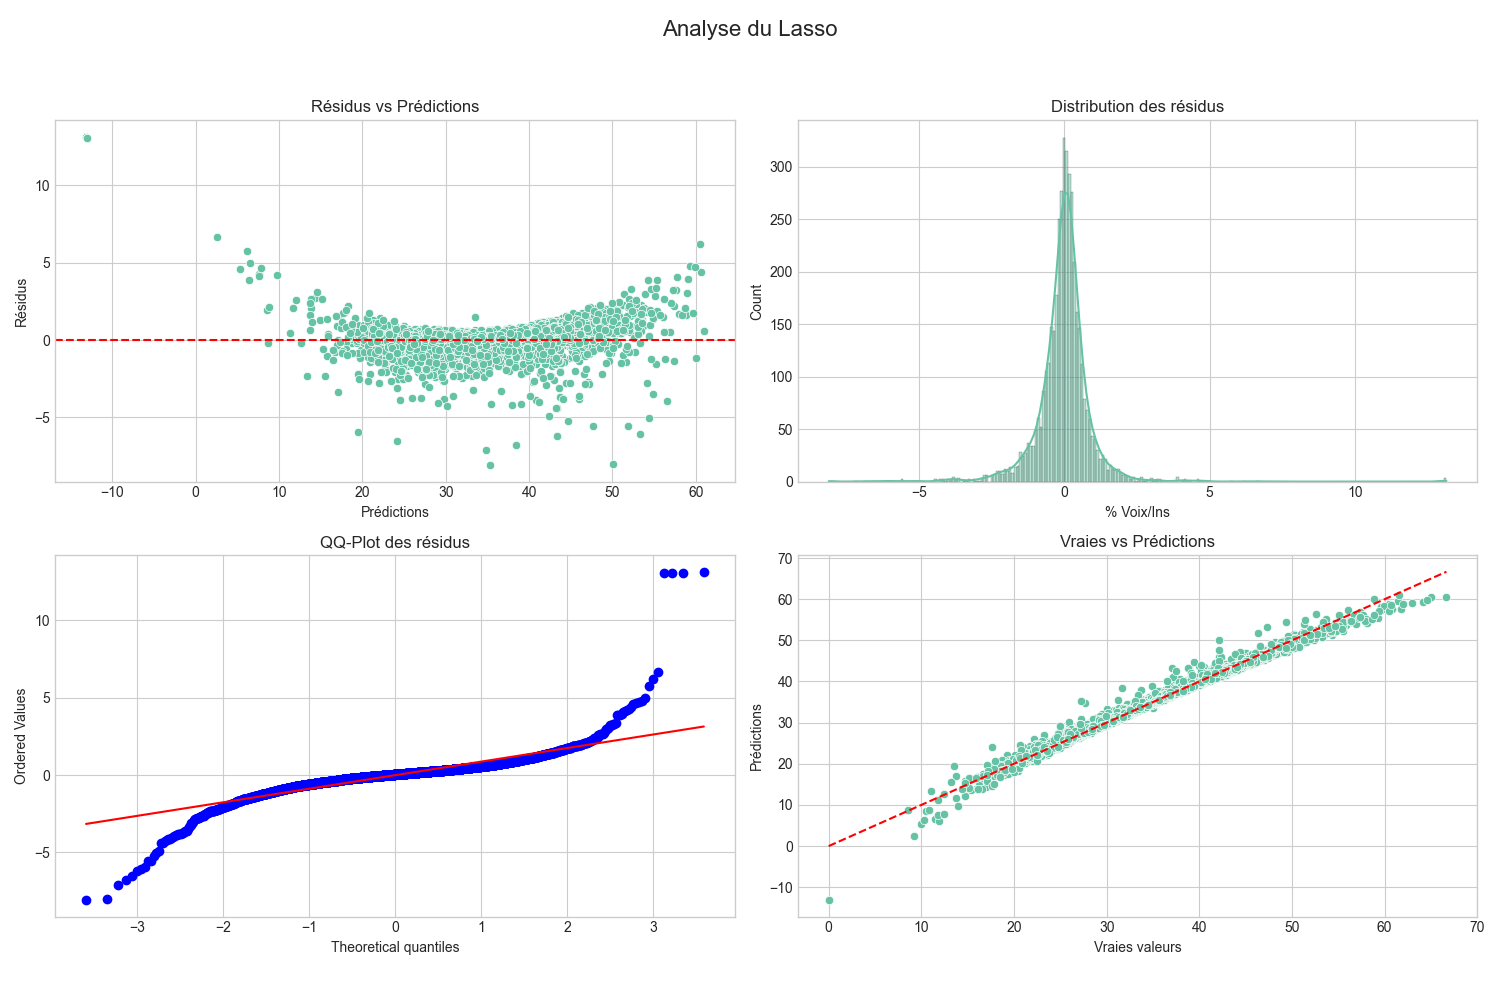
\includegraphics[width=0.8\textwidth]{figures/graphs_analyse_model_Lasso.png}
        \end{center}
    
    \end{frame} 

              
        
    \begin{frame}{XGBoost}
        \begin{center}
            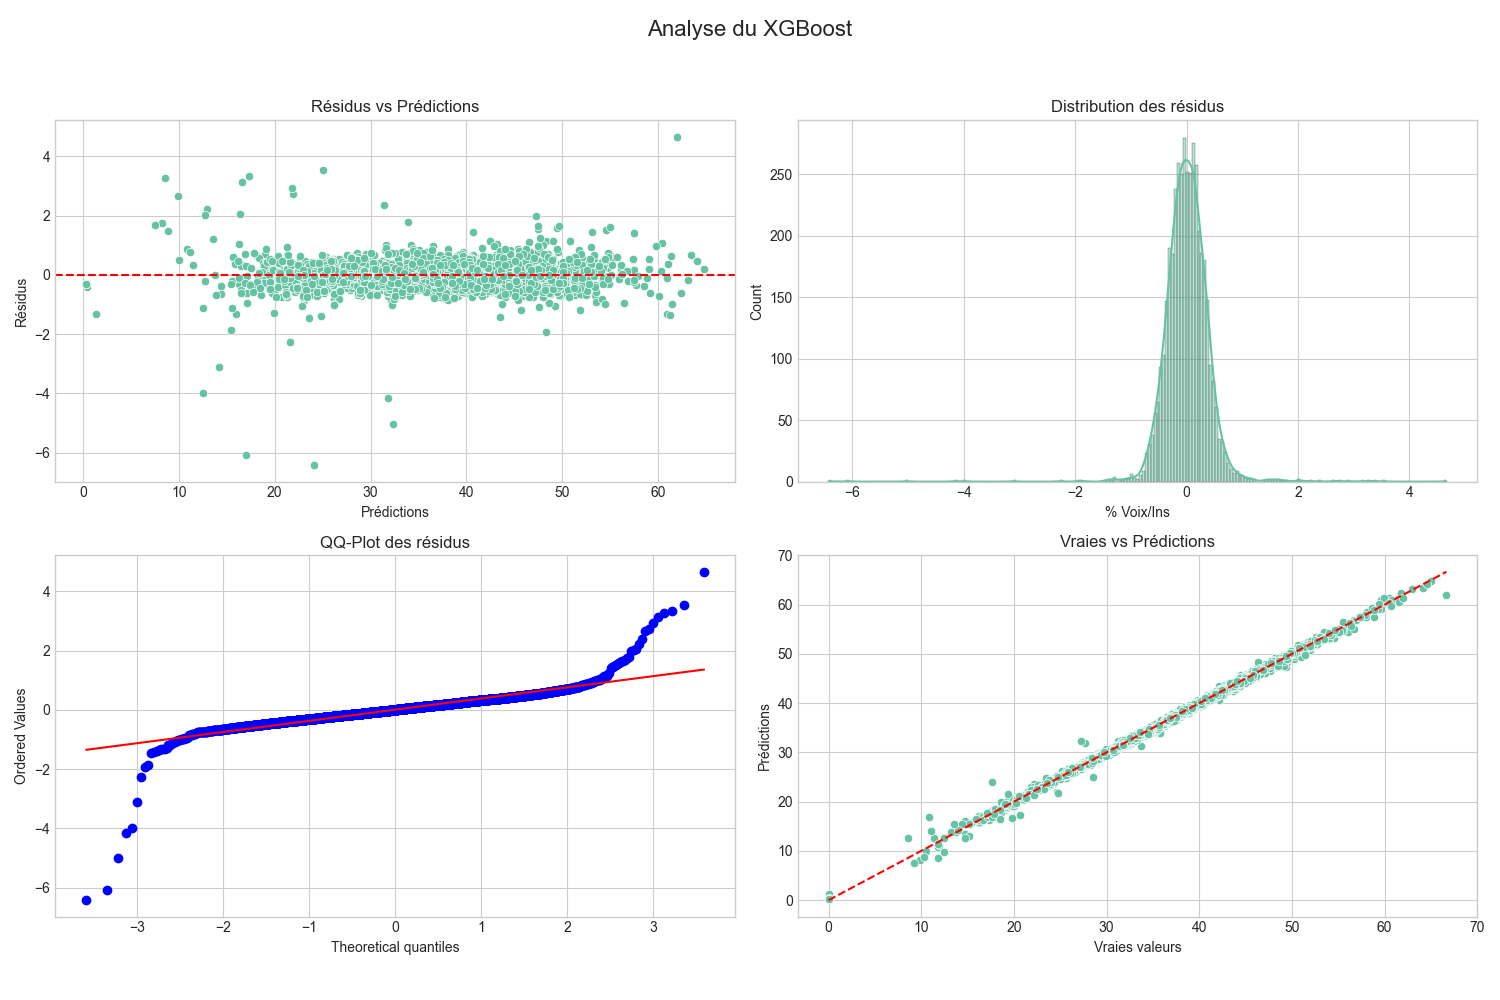
\includegraphics[width=0.8\textwidth]{figures/graphs_analyse_model_XGBoost.png}
        \end{center}
    
    \end{frame}    
        


\begin{frame}[allowframebreaks]{Interprétation des graphiques}
    
    les QQ-plots des résidus :  vus qu'ils représentent les quantiles d'une distribution normale théorique vs ceux observés , et comme les deux modèles ont des courbes en 'S' très applaties et presque centrée sur la diagonale , ont en conclut que 'les résidus des deux modèles on une distribution  presque normale '
                
    \framebreak        
    Histogrames des résidus : la différence notable , ce sont l'intervalles sur lesquels ils s'étalent :
        \begin{itemize}
            \item[.] ceux de XGBoost s'étalent de -6 à 6
            \item[.] ceux de Lasso s'étalent de -11 à 11
        \end{itemize}

        cela veut dire que les erreurs de Lasso varient beaucoup (prennent des valeurs plus ) plus que ceux de XGBoost , donc XGBoost est préférable comme modèle

    \framebreak

    \textbf{ Residus vs Prédictions} : les graphiques montres que les residus de XGBoost sont plus concentrés autour de zero que ceux de Lasso . On ve
    
    \framebreak

    \textbf{}
\end{frame}


\subsection{Importance des features}
\begin{frame}[allowframebreaks]
\frametitle{Les meilleurs features pour Lasso}
    un premier truc

    \framebreak
\end{frame}


\end{document}